\documentclass[11pt]{article}

\usepackage{algorithm2e}
\usepackage{algorithmic} 
\usepackage{amsmath}
\usepackage{amsthm}
\usepackage{booktabs}
\usepackage{dcolumn} 
\usepackage{epstopdf}
\usepackage{fourier}
\usepackage{fullpage}
\usepackage{graphicx}
\usepackage{hyperref}
\usepackage{longtable} 
\usepackage{natbib}
\usepackage{rotating}
\usepackage{tabularx}

\hypersetup{
  colorlinks = TRUE,
  citecolor=blue,
  linkcolor=red,
  urlcolor=black
}

\begin{document} 

\newtheorem{prop}{Proposition}

\title{Peer-to-Peer Rental Markets: \\ Some Simple Economics of the ``Sharing Economy''} 

\date{\today}

\author{John J. Horton \\ Leonard N. Stern School of Business \\ New York University\footnote{ Author contact information, datasets and code are currently or will be available at \href{http://www.john-joseph-horton.com/}{http://www.john-joseph-horton.com/}. } }
\maketitle

% \begin{table} 
% \caption{Research Questions for the Sharing Economy} 
% \begin{tabular}{ll} 
% Is the sharing economy efficient? Is it just regulatory arbitrage? \\  
% What happens to government revenue? \\ 
% Can a P2P rental market emerge when everyone already owns? When no one owns? \\ 
% How does a reduction in transaction costs affect all of the findings? \\ 
% What consumer goods are most amenable to P2P sharing? \\ 
% Does the emergence of sharing cause product market demand to rise or fall? \\ 
% Does sharing increase efficiency? When are the gains the largest? \\ 
% What does sharing do to product market demand curve for the good?\\  
% In the presence of sharing, what is the distribution ownership? \\ 
% What fraction of goods might be shared? \\
% What does sharing do to the elasticity of demand?\\  
% What happens when capital ownership is paired with owner-supplied labor? \\ 
% Does sharing allow any markets that would not otherwise exist to now exist? \\ 
% What are the comparative statics of changes in individual valuations of a good and the gap between those valuations?\\ 
% How does the model change when there are different numbers of the different types? \\
% Are firms at a disadvantage? \\
% \end{tabular} 
% \end{table} 

% \begin{table}
% \caption{Sharing Economy Research questions}
% \centering
% {\footnotesize 
% \begin{tabular}{llp{8cm}} 
% \toprule
% Topic & Research Question & Model prediction \\ 
% \hline 
% {\bf Product market} \\ 
% & What goods are amenable to P2P rental? & TK \\ 
% & Effect of P2P rentals on the product market price in the long-run & TK \\
% & Long-run elasticity of demand & TK \\ 
% & Why did the firm sell rather than rent? & TK \\    
% {\bf Welfare} \\ 
% & Prior-owners not renting out & TK \\ 
% & Prior-owners now renting out & TK \\ 
% & Prior non-owners now renting & TK \\
% & Efficiency & TK \\ 
% {\bf Rental rates} \\
% & What is the short-run rental rate? & TK \\
% & What is the long-run rental rate?  & TK \\ 
% {\bf Participation} \\ 
% & Who rents out in the long- and short-run? \\ 
% {\bf Comparative statics---Transaction Costs} \\ 
% & long-run rental rate & TK \\ 
% & long-run product market price & TK \\ 
% & Ownership shares & TK \\ 
% \bottomrule
% \end{tabular}  
% }
% \end{table}


\begin{abstract}
\noindent  
Recently a number of computer-mediated peer-to-peer (P2P) rental markets in durable consumer goods have emerged. 
In this paper, I present a simple model where consumers that differ in their planned usage (and hence ownership decision) about goods creates the potential for P2P trades. 
I compare a short-run where existing owners can rent to non-owners and a long-run where all consumers can revise their ownership decisions. 
The model makes several predictions. 
First, to support a P2P rental market, product market prices have to be low enough that some people buy, but not so low that everyone buys: 
the existence of non-owners that still value that good is what generates the demand. 
Market clearing in the short-run comes from owners and renters economizing on use---though a glut is possible if spare owner capacity exceeds non-owner demand even when the rental rate is zero. 
Market clearing in the long-run comes as consumers revise their initial ownership decisions in light of the possibility of sharing.  
In long-run, consumers are indifferent between renting and owning---they consume the same amount of the good at the same cost. 
Most commentators have implicitly assumed that P2P rental markets will reduce total ownership, but a sharing economy ``Jevon's paradox'' is possible in which the emergence of P2P rentals stimulate greater ownership---namely if the short-run rental rate is greater than the product market price, consumers will be drawn into ownership.   
I also consider the comparative statics from technological innovations that reduce transaction costs and explore what goods are particularly amenable to rental. \newline 
\noindent JEL J01, J24, J3
\end{abstract} 

% http://www.forbes.com/pictures/ehfk45edlgh/0122_sharing-williams-snapgoods_650x455-jpg/
% http://www.zdnet.com/the-sharing-economy-that-doesnt-exist-7000030137/
% http://www.economist.com/news/leaders/21601257-too-many-obstacles-are-being-placed-path-people-renting-things-each-other-remove
% http://meshing.it/
% These cites have lowered the opportunity cost r
% http://petapixel.com/2013/07/16/camera-gear-rentals-is-big-business-and-lensrentals-proves-it/ 
% www.salon.com/2013/09/17/the_sharing_economy_muscles_up/
% http://techcrunch.com/2012/02/27/following-thefts-luxury-car-sharing-service-higear-acquired-by-rent2buy/
% http://poshmarkapp.tumblr.com/post/73422383633/poshmark-s-closet-sharing-economy-report 
% http://www.forbes.com/sites/tomiogeron/2013/01/23/airbnb-and-the-unstoppable-rise-of-the-share-economy/

% Popular Books
% http://www.amazon.com/Mesh-Why-Future-Business-Sharing/dp/B00A16VVX8
% % http://www.amazon.com/Whats-Mine-Yours-Collaborative-Consumption/dp/0061963542/ref=pd_cp_b_0 

% From the Forbes article: 
% ``Additionally, GM can incentivize sales by promoting the idea that a new car can now come with a rental income stream attached.'' 


% “We’re going to have to invent new economics to capture the impact of the sharing economy,” says Arun Sundararajan, a professor at the Stern School of Business at NYU who studies this phenomenon. The largest question for academics is whether this all creates new value or just replaces existing businesses.

\section{Introduction}
Peer-to-peer (P2P) rental markets have recently sprung up for a variety of durable goods:
examples include cars, lodging, clothing, tools, bicycles, cameras, offices, parking spaces and so on.
These new marketplaces are invariably computer-mediated, with the facilitating platform taking steps to reduce the transactions costs that presumably make these kinds of exchanges heretofore unprofitable to run. 
Perhaps the most prominent example of P2P rental markets is Airbnb, which allows individuals to rent out spare bedrooms, apartments or even entire homes.
 
These emerging P2P rental markets are viewed by some as a the first signs of a seachange in consumerism: 
this so-called ``sharing economy'' might expand access to goods, increase efficiency by increasing utiliziation, reduce ownership and provide more ways for individuals to earn an income. 
Aside from the business interest (these sharing economy companies have received at least TK billion in VC investment), these companies have also attracted (mostly negative) policy interest. 
Critics charge that their primary competitive advantage of these peer-to-peer lenders is regulatory arbitrage: 
sellers in these markets---not subject to the same regulations as conventional firms---can price their goods artificially (and inefficiently) cheap. 

%% Car-sharing services like RelayRides, Uber, Sidecar and Lyft have repeatedly encountered regulatory resistance from nearly every city they have begun operations in, with that opposition often spearheaded by existing Taxi companies.   
%% Airbnb was---until recently---in a protracted fight with the New York Attorney General's office regarding hosts potential violation of New York City's illegal hotel laws.  
%% Further, critics argue that the renters in these markets are responding to harsh economic conditions and that they would not participate if there was a better economy. 

% \subsection{Ramesh Notes} 
% - Need to prove the uniqueness of equilibria 
% - How does depreciaation enter in? it's now a fixed cost for renters 
% - In the long-run, for the same market price p, the product market demand is less elastic because the marginal buyer can not receive rental income, which rises with the product market price. It's not completely offsetting, 
% - If product market demand less elastic, if the products have market power product market prices should rise.  
% - To owners to fully internalize benefits?    

The purpose of this paper is to explore these arguments through the lens of a simple model of a durable goods product market before and after the introduction of P2P rentals. 
In the model consumers decide whether to buy a good based on how much utility it would bring them. 
Utility in turn depends on how much the good would be used if purchased.
I assume that all goods offer declining marginal utility from usage and that eventually utility would go below zero. 
If the utility from the optimal level of usage is greater than the purchase price, the consumer buys the good. 
Even in the absence of any direct marginal usage cost, individuals will generally not use a good 100\% of the time. 
For example, a hobbyist guitar owner might play 5 hours a week, but few would play 50 voluntarily and 100 hours a week would for almost everyone be hellish.
This aspect of ownership---a usage rate often (far) below 100\%---combined with a sufficient number of non-owning consumers that still value the good---is what creates the economic rationale for P2P rental markets.      

The general characteristic of goods that are ``rentable'' are those that are used infrequently but are expensive: 
cars and hotels in distant cities, tuxedos, certain tools, etc.
However, these goods were usually offered by a company who owned the stock with the explicit purpose of renting.  
And although individuals are owned by at least some consumers who would have excess capacity, the transaction costs of facilitating peer-to-peer rentals would be prohibitive
Simply finding an appropriate trading partner would be difficult, to say nothing of coming to terms, writing a contract, monitoring compliance, handling disputes, making payment and so on. 
Further, those individuals that owned a good despite the existence of a rental market were likely those with relatively little excess capacity to rent out. 


\begin{table}
\caption{Sharing economy companies and the category of goods of services used}
\centering
\begin{tabular}{ll} 
\toprule
Good or Service & Company \\ 
\hline 
Short-term lodging   & Airbnb, VRBO, Couchsurfing  \\ 
Cars            & UberX, Lyft, RelayRides, Sidecar, Getaround  \\   
Parking         & Park Circa, ParkatmyHouse, Parking Panda \\
Bicycles        & Liquid \\   
WiFi Router     & Fon \\ 
Boat            & Boatbound \\
Camera equipment& LensRentals  \\  
Household goods & SnapGoods   \\ 
Kennel          & DogVacay    \\ 
Clothes         & GirlMeetsDress \\
\bottomrule
\end{tabular}  
\end{table}

There are several economic questions that this creation of peer-to-peer rentals raise. 
Does the product market demand for the durable good go up or down when P2P rental markets emerge?  
What determines the connection between the produce market price and rental rate in the long- and short-runs? 
How does the possibility of rental affect the elasticity of demand for the product? 
What are the welfare consequences for consumers? 
How does initial pattern of good ownership and how does it change? 
What goods are particularly amenable to sharing and why?  

To answer these questions, I develop a simple model that starts with a collection of would-be consumers for a good that make a purchasing decision before the possibility of rental.
Consumers consider the indirect utility from their chosen level of intensive-margin consumption and compare it to the purchase price. 
Those whose indirect utility is increased buy the good, while those that do not go without.  
I assume that a technological shock creates the possibility of owners renting out their excess capacity to non-owners. 
This creates a ``short-run'' P2P rental market in which equilibrium is defined by a rental rate that clears the market among existing owners and non-owners. 
I consider a ``long-run'' where owners and renters can revise their purchase decisions.  
If the short-run rental rate is below the purchase price plus the costs of renting, then ownership is less attractive, which will reduce \emph{purchase} demand for product, lowering prices. 
However, if the rental rate is above the purchase price plus the cost of renting, ownership becomes more attractive, increasing demand and raising purchase prices in the product market. 

The revision in the ownership decision in the long-run potentially affects product market demand. 
I consider how these product price changes impact welfare and compare them to product market price changes in the absence of P2P rentals. 

One issue that is initially ignored are transaction costs, reset costs and depreciation. 
I modify the basic framework to include these costs and consider how it changes the results. 
One of the main findings is that when transactions costs are sufficiently high, the P2P rental market cannot exist. 
This finding suggests that the technological changes---namely the maturation and increasing penetration of the Internet and web-based technologies---were the technological shock that made these P2P rental markets feasible. 

After the theoretical analysis, I present some results from a survey designed to explore some of the assumptions and predictions of the model. 

Goods with high purchase prices but low and predictable intensive margin usage are ideal for P2P rental markets: 
the purchase price is high enough that there are lots of would-be consumers with high willingness to pay and enough owners with excess capacity that the market-clearing rental rate is not prohibitively high. 
When produce market prices are low, there is no excess demand so nearly everyone buys the product, so even if the good is used infrequently, no rental market can exist.  
For example, there is no rental market in egg timers---although they are used infrequently and quite durable, there is neither supply (no one owning finds it worth the trouble to rent them out) nor demand (if one wants one, they go to the product market). 
Other goods are expensive but there is no excess capacity, as they are used more or less continuously. 
For example, there is and can be no P2P rental market in dentures. 
Other goods are used infrequently and are expensive but make poor sharing candidates because demand is so unpredictable. 
For example, a back-up gas-powered electrical generator is used infrequently but would be difficult to rent in a P2P market, as demand is likely to be correlated in space and time. 

\section{Consumer's decision about how intensively to use a good} 
Consider a consumer that has to decide how much of their time to allocate to the use of some purchased durable good. 
Their money-denominated utility function is
\begin{equation}
u(x) = 2 \alpha x - x^2  
\end{equation} 
where $x \in [0,1]$ is the fraction of time they spend using the good, $\alpha \in (0,1)$ is a parameter for how much utility they derive from the good. 
Individual intensive margin ``demand'' is  
\begin{equation}
x^* = \alpha  
\end{equation} 
and indirect utility is 
\begin{equation}
v(\alpha) = u(x^*) = \alpha^2.  
\end{equation} 
The good costs $p$ to own, and so a forward-looking consumer will buy if 
\begin{equation} 
\alpha^2 > p. 
\end{equation} 
Note that for all $\alpha^2 > p \wedge \alpha < 1$, the consumer will have an amount of time $1 - x^*$ when they are not using the good.

\subsection{Three consumption possibilities with two consumer types} 
Consider a marketplace with two consumer types that are equally common: $\alpha_H$ and $\alpha_L$ with $\alpha_H > \alpha_L$. 
For a given price $p$, there are three market possibilities: 
everyone buys: $\alpha_L^2 > p$; high-types buy but low-types do not: $\alpha_H^2 > p > \alpha_L^2$; and no one buys when $\alpha_H^2 < p$. 
This gives a market demand curve of 
\begin{equation}
   D(p) = \left\{
     \begin{array}{ll}
       0 & : p > \alpha_H^2\\
       1 & : \alpha_H^2 \ge p > \alpha_L^2  \\
       2 & : p \le \alpha_L^2  \\
     \end{array}
   \right.
\end{equation} 
Figure~\ref{fig:three_types} illustrates the possibilities by plotting regions on the the space of $\alpha_H \in [0,1] \times \alpha_L \in [0,1]$ when $p = 0.5$.  
The upper-right triangle is the region where both consumer-types buy and the lower-left triangle where neither buy: 
the cross-hatched rectangle shows the area where high-types buy but low-types do not. 
In the cross-hatched rectangle where high-types buy and low-types do not, there is a possibility of mutually beneficial trade:
the low-types here have $\alpha_L > 0$ and hence value the good and the high-types have $x^* < 1$, which gives them some excess capacity to rent out. 

\begin{figure}
\centering 
\caption{Three consumer market possibilities in the absence of P2P rental with two consumer types}
\label{fig:three_types} 
\begin{minipage}{0.8 \textwidth} 
\includegraphics{./images/three_parts.pdf} 
\end{minipage}  
\end{figure} 

\subsection{Short-run P2P rental equilibrium} 
We now suppose that through some technological advance, it becomes possible for the high-types to costlessly sell their entire excess capacity to the low-types. 
We will define the resulting P2P rental market as being in a short-run equilibrium, in that---at first---no consumer can revise their ownership decision. 
Before the possibility of rental, the high-types were simply consuming $\alpha_H$, giving $1-\alpha_H$ to rent out.
If they owned the good, the low-types would consume $\alpha_L$. 
However, with the new possibility of rental, each consumer's decision problem has changed. 
The new owner optimization problem---when the rental rate is $r$---is 
\begin{equation}
\max_x \quad 2\alpha_H x - x^2 + (1-x)r - p,   
\end{equation} 
whereas the renter optimization problem is 
\begin{equation}
\max_x \quad 2 \alpha_L x - x^2 - xr.  
\end{equation} 
Both decision problems yield the same usage decision: 
\begin{equation}
x^*_i = \left\{
     \begin{array}{ll}
       \alpha_i - r/2 & : 2\alpha_i > r \\
       0 & : \mbox{else}  \\
     \end{array}
   \right.
\end{equation} 
For the rental market to clear 
\begin{equation} 
1 - x^*_H(r) = x^*_L(r)
\end{equation}   
which implies that 
\begin{equation} \label{eq:strr} 
r = \alpha_H + \alpha_L - 1.  
\end{equation} 
Because only positive rental rates are possible, a glut can exist if $\alpha_H + \alpha_L < 1$: a negative rental rate would be needed to ``clear'' the market.
In contrast, when $\alpha_H + \alpha_L > 1$, both owners and renters need to economize on their usage of the good until the market clears.   
Figure~\ref{fig:market_clearing} illustrates market clearing: 
In the absence of the P2P rental market, each user consumes $\alpha$ according to their type. 
At first, the high-types user $x^*$, indicated with a light, 45 degree line . 
For short-run market clearing, the high-types economize on usage (heavy line) until $1-x_H^*(r) = x_L^*(r)$. 

\begin{prop}
If all consumers were allocated the good, if their cumulative usage would exceed the full utilization capacity of the actual stock of purchased goods, then a positive rental rate is needed to clear the market. 
\end{prop} 

\begin{figure}
\caption{Market clearing with two consumer types in a P2P rental market} 
\centering
\label{fig:market_clearing} 
\begin{minipage}{0.90 \linewidth}
\includegraphics{./diagrams/market_clearing.pdf}
\end{minipage} 
\end{figure}

\begin{prop}
If the marginal utility of either type goes up ($\alpha_H$ or $\alpha_L$ increase), short-run rental rates increase. 
\end{prop} 

\subsection{Consumer welfare in the short-run} 
For a renter, indirect utility under the short-run P2P rental equilibrium is
\begin{eqnarray} 
v_R(\alpha_L, r) &=& \frac{1}{4}\left(r - 2\alpha_L \right)^2  \\
                 &=& \frac{1}{4} \left[ (1-\alpha_H) + \alpha_L \right]^2
\end{eqnarray} 
which is always positive. 
Note further that the renter's increase in utility from the P2P-rental market is proportional to the square of their own (hypothetical) consumption and the high-types \emph{non}-consumption in the absence of the rental market. 
In other words, for renters, the most value is unlocked when they had high latent demand unmet demand for the good and when there was a great deal of ``wasted'' excess capacity from the high-types. 
Not further than the most value is created for sellers when $\alpha_H = \alpha_L + \epsilon$ (since $\alpha_H > \alpha_L$) i.e., valuations are nearly identical, though this condition also makes it unlikely for a P2P rental market to emerge from an existing high-types buy/low-types do not because it requires $p$ take a very specific value, namely $p \in (\alpha_L, \alpha_L + \epsilon]$. 

For the owner of a good, their pre-rental market indirect utility was $\alpha_H^2$. 
The increase in utility from the emergence of the P2P rental market, $\Delta v_O = v_O(\alpha_H, r) - \alpha_H^2$ is  
\begin{eqnarray} 
\Delta v_O &=& \left( \frac{3}{4} (1-\alpha_H) + \frac{1}{4} \alpha_L \right) (-1 + \alpha_H + \alpha_L)  \\
                 &=& \left( \frac{3}{4} (1-\alpha_H) + \frac{1}{4} \alpha_L \right) r   \\
                 &>& (1-\alpha_H)r 
\end{eqnarray} 
As we would expect, any increase in utility depends upon having a positive rental rate. 
We also know that this is only the case if $1- \alpha_H < \alpha_L$ and so $\Delta v_O > (1-\alpha_H)r$. 
In other words, the increase in utility for the owner is always greater than simply selling the $1-\alpha_H$ at $r$. 
The economic intuition is that when there is an excess of demand, the owner can optimally economize their own consumption to increase their utility beyond just not adjusting own-consumption and selling the excess.  

\begin{prop}
An increase in $\alpha_H$ has an ambiguous effect on the increase in welfare from P2P rental. 
\end{prop} 
\begin{proof}
TK---weak. 
If $\alpha_L < 3/4$ and $\alpha_H > 1 - \frac{\alpha_L}{3}$, which implies that $\alpha_H > 3/4$, an even higher $\alpha_H$ implies a smaller increase in utility from the emergence of the P2P rental market. 
In other words, if there is relatively little latent demand (low $\alpha_L$) and a high consumption utility for the high-types (high $\alpha_H$), an increase in $\alpha_H$ reduces the gain: 
the utility from consumption is a wash and less can be sold, even though the rental rate is a bit higher.
Alternatively, if $\alpha_L > 3/4$, a further increase in $\alpha_L$ does raise the rental rate more, but it also makes providing more supply costlier.  
\end{proof} 

\begin{prop}
An increase in $\alpha_L$ increases the owner's surplus from the emergence the P2P rental market. 
\end{prop} 
\begin{proof}
Unsurprisingly, an increase in $\alpha_L$ simply increases demand for the owner's excess capacity and so the increase in utility is proportional to the owner's capacity, $1-\alpha_H$ and the latent demand from the low-type, $\alpha_L$.  
\begin{equation}
\frac{\partial \Delta v_O}{\partial \alpha_L} = \frac{1}{2} \left[(1-\alpha_H) + \alpha_L \right] > 0.  
\end{equation} 
\end{proof} 

\begin{prop}
An owner's utility is increasing in the $\alpha$ and increasing in the rental rate, $r$. 
\end{prop}

\begin{prop}
Regardless of the rental rate, an owner has a higher utility with the existent of the P2P rental market assuming there is no change in the product market price for the good. 
\end{prop}

\subsection{Long-run P2P rental equilibrium} 
In the long-run equilibrium, all parties can revise their ownership decisions. 
The return to owning is 
\begin{equation}
v_{O} = 2\alpha_i x^* - x^{*2} + (1-x^*)r_{LR} - p   
\end{equation} 
whereas the return to renting is 
\begin{equation}
v_{R} = 2\alpha_i x^* - x^{*2} - x^*r_{LR}.  
\end{equation} 
\begin{prop}
In the long-run P2P rental equilibrium, the rental rate equals the product market purchase price and ownership does not depend on usage patterns.  
\end{prop}
\begin{proof} 
The first order condition in both scenarios is $2 \alpha_i - 2 x_i - r_{LR} = 0$ and so $x^* = \alpha_i - r/2$. 
Using this solution to compute the indirect utility, we get 
$v_O = \alpha ^2-p+\frac{r^2}{4}-\alpha  r+r$ and $v_R = \frac{1}{4} (r-2 \alpha )^2$. 
Setting $v_O = v_R$, the $\alpha$ term drops out and we are left with $p = r$. 
\end{proof} 

\begin{prop}
The fraction of consumers owning in the long-run is the average usage rate in the population.  
\end{prop} 
\begin{proof} 
Let $\gamma$ be the fraction of consumers that purchase the good in equilibrium. 
For the market to clear, 
\begin{equation}
\gamma \left[ (1-x_H(p)) + (1-x_L(p))\right] = (1-\gamma)\left(x_H(p) + x_L(p) \right) 
\end{equation} 
which simplifies to 
\begin{equation}
\gamma = \frac{x_H(p) + x_L(p)}{2}.  
\end{equation} 
\end{proof} 
The new long-run product market demand curve is thus
\begin{equation}
D(p) = \alpha_H + \alpha_L - p.  
\end{equation} 

Before the short-run equilibrium arose, when high-types bought and low-types did not, demand was $1$. 
$\alpha_H^2 > p$ and $\alpha_L^2 < p$. 

\subsection{Sharing economy ownership ``paradox''} 
Jevon's paradox was based on the empirical observation that increased demand tended to, in the long-run, decrease prices. 
There is the possibility of analogous ``paradox'' can occur with the sharing economy, in that the existence of a competitive P2P rental market can stimulate \emph{ownership}.   
For economic intuition, consider the couple that decides to purchase a second home with the expectation that they can partially recoup their outlay via Airbnb or VRBO. 

To see whether the emerging of P2P rentals will increase or decrease total ownership, we need to consider whether the short-run rental rate defined by Equation~\ref{eq:strr} is greater than or less than the purchase price. 

\begin{prop}
If the market-clearing short-run rental rate is above the purchase price, ownership will increase, otherwise decrease. 
\end{prop} 

\begin{prop}
An increase in the product market price reduces owner welfare with and without the P2P rental market, but the reduction in welfare is smaller in magnitude in the P2P rental case than in the non-rental case (where the reduction is 1 for 1). 
\end{prop}
 
\begin{prop} \label{prop:paradox} 
Sufficiently high usage valuations and a sufficiently low product market purchase price can cause total ownership to increase with the introduction of P2P rental markets.  
\end{prop} 
\begin{proof}
In terms of the model, an increase in ownership occurs when the short-run rental rate is greater than the purchase price, or $r_{SR} > p$. 
This occurs when $r_{SR} = -1 + \alpha_H + \alpha_L > p$. 
We can re-write the paradox condition as  
\begin{equation} 
\alpha_H > 1 + p - \alpha_L  
\end{equation}
which is more likely to be satisfied with higher valuation parameters and lower purchase prices.   
\end{proof} 

The economic intuition for Proposition~\ref{prop:paradox}  is straightforward: 
with high values of $\alpha_H$ and $\alpha_L$, there is a higher level of demand (from the low-types) and less supply (from the high-types), which makes ownership more attractive. 
A higher purchase price makes the paradox less likely for the simple reason that a purchase is more expensive. 
Note that the paradox cannot occur regardless of the purchase price is $\alpha_H + \alpha_L < 1$, which means that the high-types must---in the absence of the P2P rental market---use the good more than 1/2 the time. 
This is partly due to our modeling convention of their being equal numbers of both types---if low-types were far more numerous, then the equivalent paradox condition could be more easily met: 
consider that there are far more people that take vacations than their are people considering owning a second home.  

\subsection{Consumer welfare under changes in the product market price} 
If the conditions specified in Proposition~\ref{prop:paradox} are satisfied, then demand in the product market increases. 
This higher product market price could undo some of the welfare gains from P2P rentals. 
Let $p_0$ be the original purchase price and $p_1 = p_0 + \delta p$ be the new product market-clearing price. 
In the long-run equilibrium, this is also the rental rate. 
 

If the short-run rental rate is greater than the purchase price and ownership increases, pre-P2P owners could be made worse-off: if supply in the product market is sufficiently inelastic, then increase product market prices could offset owner gains from sharing, though TK these would partially be passed through in higher rental rates. 
\begin{equation}
\alpha_H^2 - p_0 > v(\alpha_H, r) - p_1 
\end{equation} 

\subsection{Changed product market demand curve} 
Previously, there were ``kinks'' in the product market demand curve at $\alpha_H^2$ and $\alpha_L^2$. 
In the long-run P2P rental equilibrium, product demand now varies continuously, with $D(p) = x_H(p) + x_L(p) = \alpha_H + \alpha_L - p$. 
Point elasticity of demand is now 
\begin{equation}
\epsilon = \frac{-1}{\alpha_H + \alpha_L - p} 
\end{equation} 

\subsection{Sharing and market existence} 
Prior to sharing, a sufficiently high product market price prevented a market from forming:
if $p > \alpha_H^2$, no consumer purchases the good. 
With P2P rental, does the lowest price at which some of the good is sold change?  
Proposition~\ref{prop:existence} shows that it does. 
Intuitively, if a would-be owner can monetize their unused portion, then purchasing becomes more attractive. 

\begin{prop} \label{prop:existence} 
A higher product market price is supportable with the existence of the P2P rental regime that without.  
\end{prop}
\begin{proof} 
If $p > \alpha_H^2$, no one buys the product and the market fails to exist.
The highest possible price that can support a market is $\bar{p}_{NS} = \alpha_H^2$.  
In the long-run P2P market, $D(p) = \alpha_H + \alpha_L - p$, and so $\bar{p}_{S} = \alpha_H + \alpha_L$. 
Since $\alpha_H > \alpha_H^2$ and $\alpha_L > 0$, $\bar{p}_S > \bar{p}_{NS}$.  
\end{proof} 

\subsection{Can for-profit capital-owning firms compete?} 
In the long-run P2P rental market equilibrium, there are no profits from owning to simply rent-out. 
However, owners and non-owners alike get a surplus. 
This suggests that firms that derive no consumption value from the good can not compete: 
because the consumer has excess capacity after satisfying their own consumption, they can ``profitably'' sell 
their excess capacity at any price and still have positive utility. 
A firm owning simply to rent would make zero profit. 

\subsection{Taste for diversity} 
In some formulations of the consumer problem, consumers consume some positive amount of every good offered.
For example, a Cobb-Douglas utility function has no corner solutions---every good is consumed at least a little bit.
This is obviously a large departure from empirical reality if we draw find-grained distinctions between ``goods.'' 
For example, Amazon.com currently lists 6,238 results for "blender" in the Home \& Kitchen category: 
presumably most households own far fewer than this, with most owning 1 or 0.
The reason for this pattern in the language of this model is clear: 
a consumer's $\alpha$ for Blender 2 \emph{conditional} upon owning Blender 1 is quite low and so another blender is not purchased.   
There are numerous goods that have highly negative cross price elasticities but that would not in a world of perfectly competitive rental markets in all goods.  
Very few people rent the same car they drive or vacation in their home towns. 
     
\section{Transaction costs and depreciation}

Note that in the short-run, $r$ did not depend directly on $p$, but in the long-run they are linked. 
Let $r_{SR}$ be the short-run rental rate and let $r_{LR}$ be the long-run rental rate. 
Let $p_{SR}$ and $p_{LR}$ be the short- and long-run product prices, respectively.  

If $r_{SR} > p_{SR} + \gamma$, there were excess profits available to being an owner. 
As such, in the long-run, demand in the product market will go up, raising $p_{LR}$ and lowering $r_{SR}$. 
In this case, the emergence of the sharing economy causes a Jevon's paradox of increased usage. 
Producer surplus rises, but the effect on consumers is ambiguous. 
Long-run non-sharers are made strictly worse-off, as they now face a higher price in the product market. 
All consumers that would not have purchased under the pre-sharing regime are better off, as they consumer some of the good.

TK---Prior owners now sharing have an ambiguous outcome---they consumer less and pay a higher purchase price but do receive offsetting rental income.  

On the contrary, if $r_{SR} < p_{SR} + \gamma$, ownership is less attractive and in the long-run, fewer goods will be purchased, lowering prices. 
In this case, the introduction of the sharing economy is Pareto improving with respect to consumers. 
Owners that do not rent out their good get a price reduction; former non-owners get to consume some of the good. 
For owners that rent out the good, they could consumer their old $x$ (pre-sharing) at a now-lower purchase price and so are strictly better off. 

Many goods have ``missing'' rental markets despite generating usage far below $x = 1$ because the rental rate $r$ required to cover the added transaction costs of renting would be too high to create a viable rental market. 

Suppose it costs the firm $\gamma$ to full rent-out an owned product and suppose rental goods have to be purchased in the product market. 
No arbitrage would mean that $p + \gamma = r$. 

\begin{prop}
Higher prices in the product market make the maximum transaction cost that would still permit a rental market to be lower. 
\end{prop} 

When opportunity costs are greater, people want to consumer less of each particular good, making renting relatively more attractive, meaning that a rental market can still exist with higher transaction costs. 

\subsection{What determines the fixed costs of renting?} 
Technology can reduce some of the fixed costs of renting. 
The thicker the market, the easier it is to fully make use of the excess supply. 
Goods with predictable or easily adjustable usage patterns are more likely to be P2P rental. 
Owners of vacation homes can schedule their own usage easily. 

Some goods are used infrequently, but all consumers will likely want to use them at the same time. 
A back-up generator---while infrequently used---is unlikely to make a
good P2P rental candidate, as demand spikes are likely to be correlated in both space and time. 

Reset costs presumably differ by good. 
Most things---apartments, cars, clothes etc., need to be cleaned and or serviced before they can be rented again. 
However, other goods like jewelry presumably have little reset cost.

Goods that have a high novelty value are particularly amenable to renting: 
This explains why rentals or lending of videos and books are/were commonplace.  

Goods that are difficult to transport but need to be used in a different locations will be hard to share. 
However, goods that can be used on-site by different people are more shareable. 
For example, yachts are relatively difficult to transport long distances, but there is a thriving P2P rental market in boats where many want to sail on vacation: 
in the British Virgin islands charter yachts are owned by individuals. 

If transaction costs are sufficiently high, then the rental rate would be too high to support a market (even though the high rental rate would tend to stimulate supply). 

\section{Empirical investigation} 
In conventional consumer theory, preferences over goods are assumed---the theory focuses on how those preferences are translated into purchases in light of the consumer's budget and market prices. 

\begin{figure}
\centering 
\caption{Fraction of respondents owning various quasi-durable goods}
\begin{minipage}{0.90 \linewidth}
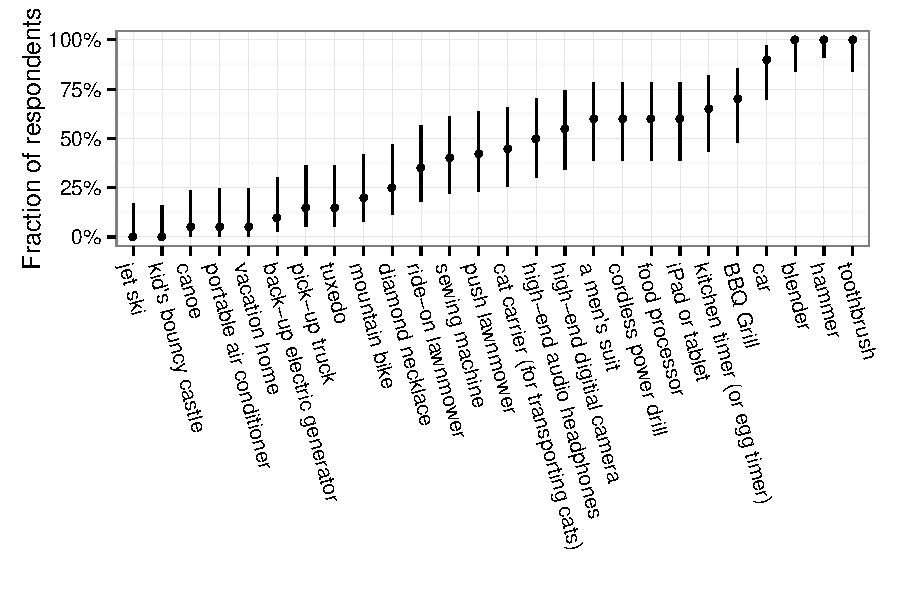
\includegraphics[width = \linewidth]{./plots/ownership_fractions.pdf} 
\end{minipage} 
\end{figure} 

Table~\ref{tab:ownership} shows that TK. 


% Table created by stargazer v.5.1 by Marek Hlavac, Harvard University. E-mail: hlavac at fas.harvard.edu
% Date and time: Thu, May 14, 2015 - 07:55:45 AM
% Requires LaTeX packages: dcolumn 
\begin{table}[!htbp] \centering 
  \caption{Respondent estimates of the fraction of time spent using a good and whether they own that good} 
  \label{tab:ownership} 
\footnotesize 
\begin{tabular}{@{\extracolsep{5pt}}lD{.}{.}{-3} D{.}{.}{-3} D{.}{.}{-3} } 
\\[-1.8ex]\hline 
\hline \\[-1.8ex] 
 & \multicolumn{3}{c}{\textit{Dependent variable:}} \\ 
\cline{2-4} 
\\[-1.8ex] & \multicolumn{3}{c}{Respondent owns the item?, ($\textsc{Own}_{ig}=1$)} \\ 
\\[-1.8ex] & \multicolumn{1}{c}{(1)} & \multicolumn{1}{c}{(2)} & \multicolumn{1}{c}{(3)}\\ 
\hline \\[-1.8ex] 
 Log estimated usage, $\log x_{ig}$ & 0.026^{**} & 0.026^{**} & 0.026^{**} \\ 
  & (0.011) & (0.011) & (0.011) \\ 
  Log household income, $\log y_i$ &  & 0.102^{***} &  \\ 
  &  & (0.025) &  \\ 
 \hline \\[-1.8ex] 
Good FE & \multicolumn{1}{c}{Y} & \multicolumn{1}{c}{Y} & \multicolumn{1}{c}{Y} \\ 
Respondent FE & \multicolumn{1}{c}{N} & \multicolumn{1}{c}{N} & \multicolumn{1}{c}{Y} \\ 
Observations & \multicolumn{1}{c}{411} & \multicolumn{1}{c}{411} & \multicolumn{1}{c}{411} \\ 
R$^{2}$ & \multicolumn{1}{c}{0.445} & \multicolumn{1}{c}{0.465} & \multicolumn{1}{c}{0.567} \\ 
\hline 
\hline \\[-1.8ex] 
\end{tabular}
\\{\footnotesize \begin{minipage}{0.75 \linewidth} \emph{Notes:}
This table reports OLS regressions where the dependent variable is an indicator for whether a respondent reported owning a particular good.
In Column~(1) the independent variable is that respondent's estimate of what fraction of their time they would spend using that good (in logs).
In Column~(2) a regressor for the log of the respondent's self-reported household income is added to the Column~(1) specification.
Column~(3) uses the same specification as Column~(1), but a respondent specific fixed effect is added. 
The sample is restricted to respondents who reports some positive amount of predicted usage of the good and reported their household income.
All regressions include good-specific fixed effects and standard errors are clustered at the good level. 
\starlanguage \end{minipage} }
\end{table}


Table~\ref{tab:ownership_attr} explores how the perceived usage attributes of the good are related to the ownership decision.
My hypothesis was that goods with an unpredictable usage pattern and/or whose usage was spread out over many small chunks would necessitate ownership. 
In Column~(1), we see that the less predictable perceived usage, the more likely the good is to be owned. 
In Column~(2), the more granular usage is, the more likely the good it to be owned. 


% Table created by stargazer v.5.2 by Marek Hlavac, Harvard University. E-mail: hlavac at fas.harvard.edu
% Date and time: Tue, Jan 26, 2016 - 07:25:30 AM
% Requires LaTeX packages: dcolumn 
\begin{table}[!htbp] \centering 
  \caption{Good usage unpredictability and chunkiness and its association with good ownership.} 
  \label{tab:ownership_attr} 
\footnotesize 
\begin{tabular}{@{\extracolsep{5pt}}lD{.}{.}{-3} D{.}{.}{-3} D{.}{.}{-3} D{.}{.}{-3} } 
\\[-1.8ex]\hline 
\hline \\[-1.8ex] 
 & \multicolumn{4}{c}{\textit{Dependent variable:}} \\ 
\cline{2-5} 
\\[-1.8ex] & \multicolumn{4}{c}{Item is owned} \\ 
\\[-1.8ex] & \multicolumn{1}{c}{(1)} & \multicolumn{1}{c}{(2)} & \multicolumn{1}{c}{(3)} & \multicolumn{1}{c}{(4)}\\ 
\hline \\[-1.8ex] 
 Unpredictability Score (US) & 0.139^{***} &  & 0.095^{***} & 0.003 \\ 
  & (0.030) &  & (0.034) & (0.034) \\ 
  Chunkiness Score (CS) &  & 0.135^{***} & 0.091^{***} & -0.018 \\ 
  &  & (0.025) & (0.029) & (0.025) \\ 
  US x CS &  &  & -0.009 & 0.006 \\ 
  &  &  & (0.018) & (0.018) \\ 
 \hline \\[-1.8ex] 
Respondent FE & \multicolumn{1}{c}{Y} & \multicolumn{1}{c}{Y} & \multicolumn{1}{c}{Y} & \multicolumn{1}{c}{Y} \\ 
Good FE & \multicolumn{1}{c}{N} & \multicolumn{1}{c}{N} & \multicolumn{1}{c}{N} & \multicolumn{1}{c}{Y} \\ 
Observations & \multicolumn{1}{c}{489} & \multicolumn{1}{c}{489} & \multicolumn{1}{c}{489} & \multicolumn{1}{c}{489} \\ 
R$^{2}$ & \multicolumn{1}{c}{0.170} & \multicolumn{1}{c}{0.169} & \multicolumn{1}{c}{0.191} & \multicolumn{1}{c}{0.500} \\ 
\hline 
\hline \\[-1.8ex] 
\end{tabular}
\\ {\footnotesize  \begin{minipage}{0.85 \linewidth} \emph{Notes:}
This table reports regressions of an indicator for whether the respondent owns a good on that same respondent's estimates of the unpredictability and granularity of usage for that good.
The two indices are normalized responses to the 1-5 scale questions on usage chunkiness and unpredictability, pooled over all respondents and goods.
Toothbrushes and backup generators are excluded from the sample. 
See Appendix~\ref{sec:survey} for the actual survey language and responses.
In each regression, a respondent-specific fixed effect is included.
Standard errors are clustered at the level of the individual respondent.
\starlanguage
\end{minipage} }
\end{table}
 

In this model presented in this paper, preferences are still primitives of the model, but they are modeled as differences in planned \emph{usage} of the good.  

\cite{kuziemko2013elastic} 

I asked a sample of respondents on Mechanical Turk various questions about a particular good: 
\begin{itemize} 
\item Does your household own a $\{$ good $\}$? (yes, no) 
\item Have you ever lent your $\{$ good $\}$ to someone else? (yes, no, n/a)
\item Have you ever rented a $\{$ good $\}$? (yes, no, n/a)
\end{itemize}  

Does planned low-usage predict non-ownership? 
If demand is not predictable, is it difficult to borrow the good? 
If a good is not owned but amenable to sharing, it is more likely to be rented? 
Do income effects matter? 

Figure~\ref{fig:usage_by_own} shows the 

\begin{figure}
\centering 
\caption{Distribution of usage indexes by ownership}
\label{fig:usage_by_own}
\begin{minipage}{0.90 \linewidth}
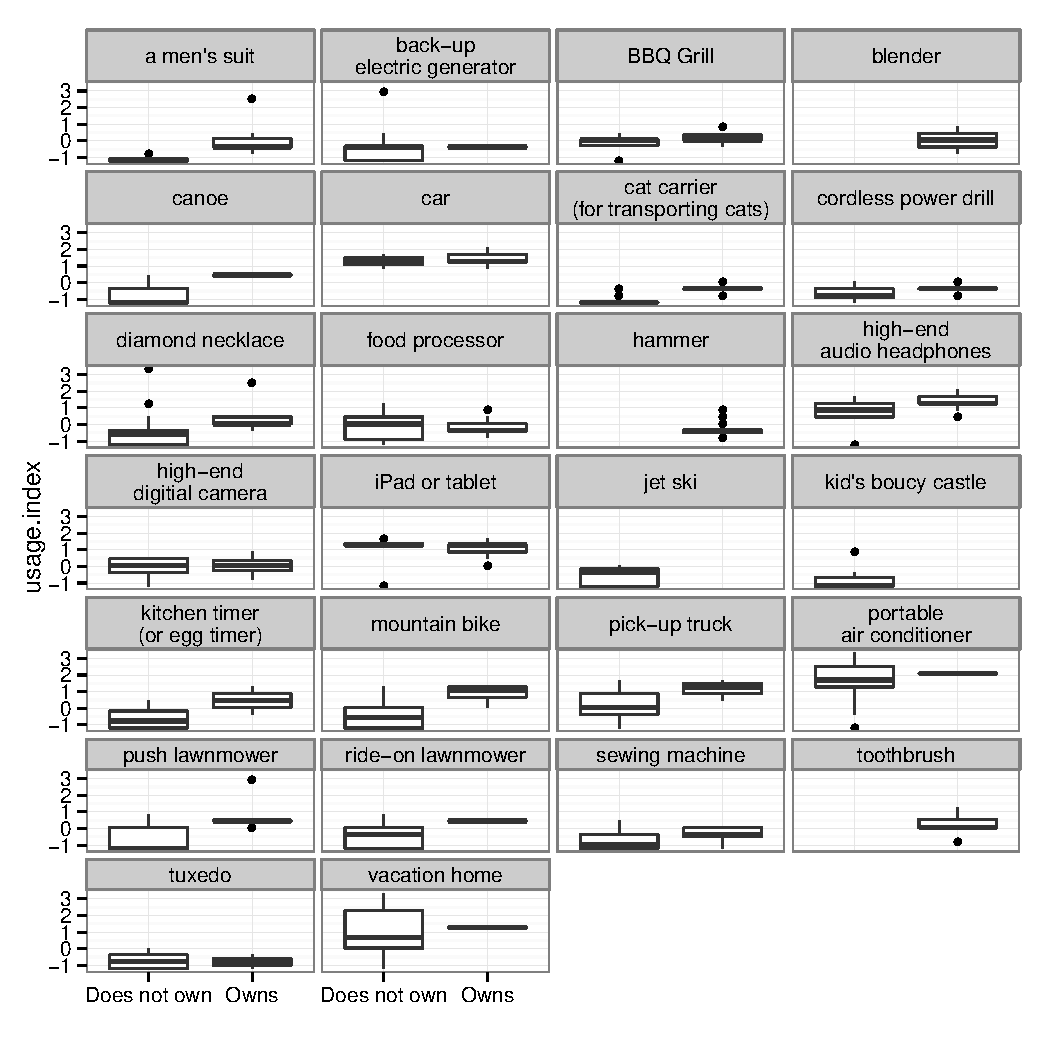
\includegraphics[width = \linewidth]{./plots/usage_by_own.pdf} 
\\
{\footnotesize
\emph{Notes:} Here are some notes. 
}
\end{minipage} 
\end{figure} 



\subsection{Reasons for non-ownership} 


\begin{figure}
\centering 
\caption{Reasons given for non-ownership}
\begin{minipage}{0.90 \linewidth}
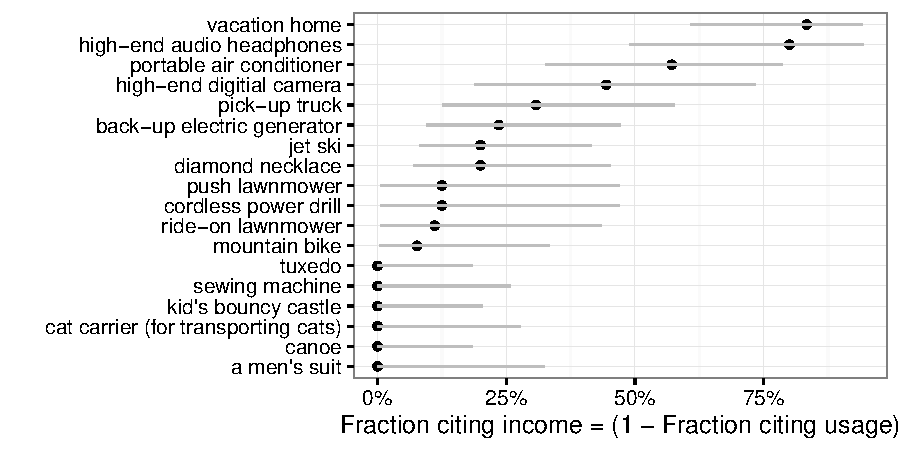
\includegraphics[width = \linewidth]{./plots/reasons.pdf} 
\end{minipage} 
\end{figure} 


\begin{figure}
\centering 
\caption{Ownership fractions by family income quartiles}
\begin{minipage}{0.90 \linewidth}
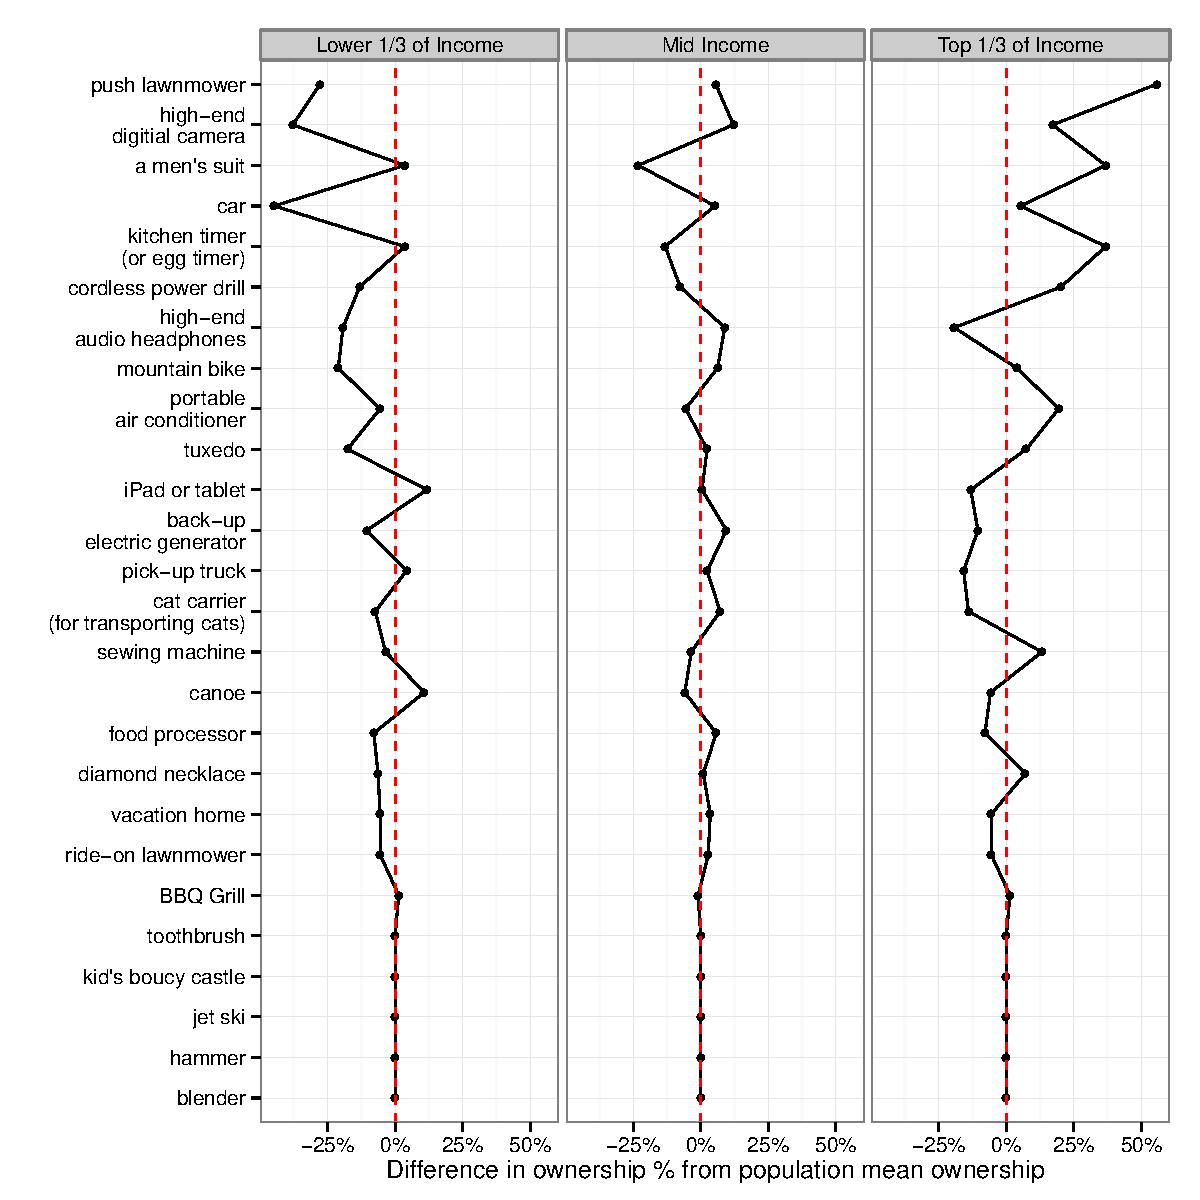
\includegraphics[width = \linewidth]{./plots/ownership_fractions_inc.pdf} 
\end{minipage} 
\end{figure} 


% <!--Lending --> 
% <b><p>Have you ever lent your ${good} to someone else?<p></b>
% <p>
% <input name="lent" type="radio" value="yes" />Yes</br>
% <input name="lent" type="radio" value="no" />No</br>
% <input name="lent" type="radio" value="na" />NA - we do not own one.</br>
% </p>

% <b><p>Have you ever borrowed a ${good} from someone else?<p></b>
% <p>
% <input name="borrowed" type="radio" value="yes" />Yes</br>
% <input name="borrowed" type="radio" value="no" />No</br>
% <input name="borrowed" type="radio" value="na" />NA - we own one.</br>
% </p>

% <b><p>Have you ever rented a ${good}?<p></b>
% <p>
% <input name="rent" type="radio" value="yes" />Yes</br>
% <input name="rent" type="radio" value="no" />No</br>
% <input name="rent" type="radio" value="na" />NA - we own one.</br>
% </p>

% <!-- Usage --> 
% <b><p>Regardless of whether your household owns a ${good}, if you did
%   own one, how much do you estimate it would be used by members of your household on average?</p></b> 
% <select name="usage"  size="1">
%   <option value="">Select one...</option>
%   <option value="0">We would not use this at all</option>
%   <option value="1" >1 minute a week (about 1 hour a year) </option>
%   <option value="2" >5 minutes a week (about 4 hours a year)</option>
%   <option value="3" >1/2 an hour a week</option>
%   <option value="4" >1 hour a week</option>
%   <option value="5" >1/2 an hour a day</option>
%   <option value="6" >1 hour a day</option>
%   <option value="7" >2 hours a day</option>
%   <option value="8" >4 hours a day</option>
%   <option value="9" >8 hours a day</option>
%   <option value="10" >16 hours a day</option>
%   <option value="11" >24 hours a day (I would continuously be using
%   this good)</option>
% </select>

% <!--Usage pattern---granularity--> 

%   <table id="likert">
%      <tr>
%          <td><input id="granularity" type="radio" name="Granularity" value="1" /></td>
%          <td><input type="radio" name="Granularity" value="2" /></td>
%          <td><input type="radio" name="Granularity" value="3" /></td>
%          <td><input type="radio" name="Granularity" value="4" /></td>
%          <td><input id="granularityEnd" type="radio" name="Granularity" value="5" /></td>
%      </tr>
%      <tr>
%          <td>Used in one big block of time</td>
%          <td></td>
%          <td>Used in a mixture of large and small blocks of time</td>
%          <td></td>
%          <td>Used in many small blocks of time</td>
%      </tr>
%   </table>


% <!-- Granularity --> 
% <b><p>
% Regardless of whether you actually own a ${good}, how do you imagine
% it would be used if it was owned by your household (on a scale of 1 to
% 5): 
% </p>
% </b>
% <select name="granularity"  size="1">
%   <option value="">Select one...</option>
%   <option value="1">1 - Used in one big block of time </option>
%   <option value="2" >2  </option>
%   <option value="3" >3 -Used in a mixture of large and small blocks
%   of time</option>
%   <option value="4" >4 </option>
%   <option value="5" >5 - Used in many small blocks of time</option>
% </select>



% <!--Usage pattern---predictibility--> 

% <b><p>
% Regardless of whether you actually own a ${good}, how predictable
% would your usage of it be if you did own it: 
% </p>
% </b>
% <select name="predictability"  size="1">
%   <option value="">Select one...</option>
%   <option value="1">1 - Very predictable---I can plan usage many weeks in advance</option>
%   <option value="2" >2  </option>
%   <option value="3" >3 -Somewhat predictable 
%   of time</option>
%   <option value="4" >4 </option>
%   <option value="5" >5 - Very unpredictable---I would never know exactly when I
%          would need to use it until right beforehand. </option>
% </select>


% <!--- Why no own --> 
% <p><b>If you do not own a ${good}, what is the primary reason?</p></b> 
% <p>
% <input name="no_own_reason" type="radio" value="na" />NA - we own one.</br>
% <input name="no_own_reason" type="radio" value="little_use" />We wouldn't use it enough to justify the purchase price</br>
% <input name="no_own_reason" type="radio" value="expensive" />We would use it, but we simply do not have the money.</br>
% <input name="no_own_reason" type="radio" value="space" />I don't have
% the space for this item</br>
% </p>


% <b><p>What is your total household income?</b>
% <select name="own_income">
%   <option value="">Select one...</option>
%   <option value="0" >Less than $10,000</option>
%   <option value="1" >$10,000-$19,999</option>
%   <option value="2" >$20,000-$29,999</option>
%   <option value="3" >$30,000-$39,999</option>
%   <option value="4" >$40,000-$49,999</option>
%   <option value="5" >$50,000-$59,999</option>
%   <option value="6" >$60,000-$69,999</option>
%   <option value="7" >$70,000-$79,999</option>
%   <option value="8" >$80,000-$89,999</option>
%   <option value="9" >$90,000-$99,999</option>
%   <option value="10" >$100,000-$149,000</option>
%   <option value="11" >More than $150,000</option>
% </select>
% </p> 



\section{Conclusion}
In the very long-run, product differentiation could move towards making sharing more attractive. 
Individuals will purchase more durable goods to reduce the frequency of replacement. 
Goods with broad appeal will see an increase in demand compared to more idiosyncratic goods that cater to the owner's taste (similar to how re-sale value enters into some consumers decisions now). 
There will be a shift towards products that are more easily shareable. 
For example, locks on cars and houses that allow remote entry will be more appealing. 

On-going technological developments should reduce the costs of sharing. 
The Internet-of-Things will make it easier to identify goods that are not being used at a moment in time. 
It will also permit more instrumentation which in turn should facilitate contracting. 
For example, many goods might make a high resolution video, with precise time-tracked location of how they are being used, reducing concerns about moral hazard. 
As more of economic and social life are computer-mediated, platforms will use this information to verify the identify and reputation of buyers and sellers, mitigating moral hazard and adverse selection.  

Product market producers will subsidize sharing of experience goods, say by offering them at a discount to known-sharers.\footnote{GM is already doing this with RelayRides}.  

For goods for which Jevon's paradox does not hold, marketing will be re-directed towards encouraging ownership.
Barring that, advertisers will trumpet the rental stream income from a purchase and highlight the advantages of residual control rights. 
We might see more B2B rentals, particular among companies that have similar inputs but are not competitors in the product market. 
Goods with declining real prices are unattractive for sharing businesses, as the trend will be towards ownership. 

Digital goods are incredibly attractive for P2P ``rental'' but since a single owner can meet all the demand among non-owners, the rental rate is zero.
The reason is that even if the owner uses $x$, $1$ is still available to the person ``rented'' to.  
Of course, this is just piracy. 

%IP-multiplexing 

\cite{sinai2005}
\cite{ikkala2014defining}
\cite{varian2000} 
\cite{byers2013rise} 
\cite{becker1965theory} 

\bibliographystyle{aer}
\bibliography{sharing.bib}

\end{document} 


%Some goods are easy to make a consumption plan for---rental homes, high-end camera equipment. 
% While it makes sense to think of consumers making an extensive margin decision---buy or not buy---their individual decision, at least for some goods, is based on a solution to another optimization problem. 
% When considering a purchase, individuals are deciding ``how much am I going to use this?'' 
% This decision has to be made for nearly every consequential purchase. 
% Once a durable good is purchased, the cost of using---less depreciation---is the opportunity cost of doing something else. 
% Once purchased, a good is used up until the point that its declining marginal utility equals only the opportunity cost. 
% This is a different decision than one makes if using a rental, where the marginal cost is both the opportunity cost and the rental rate.

% When the capital costs are very high but usage by owners is relatively low, it is more likely that there are large numbers of would-be consumers and the excess capacity to satisfy them.  
% Goods being offered my a monopolist are likely to be below the  
% Most people spent only about two minutes a day brushing their teeth, giving them 4,598 minutes they could rent out their toothbrush.  
% But reset costs are likely to be high, people want to brush around the same times each day and the price of a toothbrush is so low that anyone who brushes their teeth finds it more convenient to own. 

% % Idea: time use survey 
% Owning a good and renting it out generates costs. 
% Some of these are recognizable transaction costs, such as finding a renter and coming to terms. 
% There is also the cost of writing contracts and monitoring compliance, purchasing insurance, dealing with moral hazard and adverse selection.\footnote{High-end car company had its entire fleet of fancy cars stolen.} 

% The main effect of IT when paired with for-profit platforms are reductions in the costs of renting. 
% The platforms aggregate demand and expose where supply resides, reducing search costs. 
% They have standardize contracts. 
% They measure usage and handle payments. 
% They invest in tools to reduce information asymmetries and moral hazard. 

% % How much time was spent with a good  
% % How much that good or service costs

% What IT enables: 
% - aggregate demand 
% - expose where the supply resides 
% - overcome informational problems (information asymmetries and moral
% hazard) 
% - payment timing issues (the escrow problem) 
% - Adding complexity of moral hazard. 

% Similar to P2P electronic commerce in many respects.  Uber and Airbnb are the most prominent examples. 
% The sharing economy raises several economic questions whose answer is not intuitively obvious. 
% On the one hand, if individuals can rent infrequently used property to each other, then it seems plausible that fewer of those things are actually needed. 
% For example, it is easy to imagine one suburban neighborhood sharing a single drill, whereas before, multiple households would have purchased one. 
% Of course, rental markets are not new. 
 % On the other hand, when individuals can share durable goods among themselves the greater intensity of use may actually increase demand: 
% this ``rebound effect'' or Jevons paradox seems possible. 
% Another question is who participates in the sharing economy: 
% heavy users of some durable good are likely to purchase rather than rent, but they are also unlikely to rent the item out as they are unlikely to have much spare capacity to rent. 
% Light users do have more capacity, but they are potentially the ones that get the least utility from the good anyway. 
